\documentclass[ddcfooter, aspectratio=169, hyperref = {colorlinks,bookmarks=true,citecolor=blue,urlcolor=blue}]{beamer}
\usepackage[utf8]{inputenc}  % Kodierung der Datei
\usepackage[T1]{fontenc}  % Vollen Umfang der Schriftzeichen
\usepackage{amsmath}
\usepackage{amssymb}
%\usepackage{nameref}
\usepackage{isomath}
\usepackage{upgreek}
\usepackage{caption}
\usepackage{bbm}
\usepackage{mathtools}
\usepackage{mathrsfs}

%\usepackage{hyperref}
%\usepackage[colorlinks,bookmarks=true,citecolor=blue,linkcolor=red,urlcolor=blue]{hyperref}


\usepackage{bm}
\usepackage{bbm}

\usepackage{subfig}
%\usepackage{floatrow}

%sinnvolle Abstände im Inhaltsverzeichnis
\makeatletter
\patchcmd{\beamer@sectionintoc}
  {\vfill}
  {\vskip\itemsep}
  {}
  {}
\makeatother  

% Custom command to obtain the currently active label (of section, subsection etc.)
\makeatletter
\newcommand*{\currentname}{\@currentlabelname}
\makeatother

%Bilder neben Text
\newcommand{\lenitem}[2][.7\linewidth]{\parbox[t]{#1}{\strut #2\strut}}

\usetheme{Frankfurt}
\usecolortheme{beaver}
\setbeamertemplate{footline}[frame number]
\setbeamertemplate{navigation symbols}{}
\setbeamertemplate{headline}{}


\title[]{The Thin-Torus Limit of Fractional Chern Insulators}
\author{\texorpdfstring{\textbf {Benjamin Michen} (TU Dresden) \\ C\'{e}cile Repellin (LPMMC CNRS)\\
 Jan Carl Budich (TU Dresden), \newline \vspace{10pt} \url{benjamin.michen@mailbox.tu-dresden.de}}{}}
\date{06.09.2022}
\institute{TU Dresden}

% Insert slide with section name before each section
\AtBeginSection[]{
  \begin{frame}
  \vfill
  \centering
  \begin{beamercolorbox}[sep=8pt,center,shadow=true,rounded=true]{title}
    \usebeamerfont{title}\thesection~ \insertsectionhead\par%
  \end{beamercolorbox}
  \vfill
  \end{frame}
}




\begin{document}
\maketitle

\begin{frame}{Overview}
    \begin{columns}[onlytextwidth,T]
        \begin{column}{.45\textwidth}
           \tableofcontents[sections=1-3]
        \end{column}
        \pause
        \begin{column}{.45\textwidth}
           \tableofcontents[sections=4-5]
        \end{column}
    \end{columns}
\end{frame}

\section{What is a Fractional Chern Insulator?}

\begin{frame}
\frametitle{\insertsectionhead}
\textbf{ \large The (fractional) quantum  Hall effect\\}

 
Consider a 2D electron gas in the $x,y$-plane subjected to a perpendicular magnetic field

\begin{align}
\bm B = B \bm e_z \nonumber
\end{align}

\pause
Vector potential in Landau gauge $\bm A = (0, Bx, 0)$ yields single-particle Hamiltonian 

\begin{align}
H = \frac{1}{2 m} \left (- i \hbar \frac{\mathrm{d} x}{\mathrm{d} x}\right  )^2 + \frac{1}{2 m} \left ( - i \hbar \frac{\mathrm{d} y}{\mathrm{d} y} + eB x\right  )^2 \nonumber
\end{align}

\pause
$\Rightarrow$ Eigenenergies form perfectly flat quasi bands, so-called Landau levels

\end{frame}

\begin{frame}
	\frametitle{\insertsectionhead}
	\begin{figure}[htp!]	 
			\centering 
			\includegraphics[trim={0cm 0cm 0cm 0cm},clip, width= 0.8 \linewidth]{Images/Landau_Levels.png} 
			\caption*{Landau levels for a system of size $L_x \times L_y$.}
	\end{figure}
\end{frame}

\begin{frame}
\frametitle{\insertsectionhead}

\pause
\begin{itemize}[<+->]
	\item Complete filling of the Landau levels leads to a transverse conductance 	
	\begin{align}
	\sigma_{x,y} = n \sigma_0, \; \; \; n \in \mathbbm{N} \nonumber
	\end{align}	
	 quantized in integers of $\sigma_0 = \frac{e^2}{2 \pi \hbar}$ \\
	 \vspace{10pt}
	 \centering $\Rightarrow$ Integer Quantum Hall Effect 
	 \vspace{10pt}
	\item Filling to a fraction $\nu = \frac{1}{m}$, may lead to a fractionalized quantization
	\begin{align}
	\sigma_{x,y} =  \frac{1}{m} \sigma_0  , \; \; \; m \in \mathbbm{N} \nonumber
	\end{align}
	\centering $\Rightarrow$ \textbf Fractional \textbf Quantum \textbf Hall \textbf Effect (FQHE)
	
\end{itemize}

\end{frame}


\begin{frame}
\frametitle{\insertsectionhead}
\textbf{ \large Nature of fractional quantum Hall phases\\}
\pause
\begin{itemize}[<+->]
	\item Fractional filling leaves ``space to move''  for the particles inside the Landau level \\ $\Rightarrow$ Interactions become important
	\item FQH states are incompressible quantum liquids 
	\item They possess quasiparticle excitations acting as anyons with fractional charge 
	\item For fermions, FQH states occur at odd integer fillings $\frac{1}{3}, \frac{1}{5},...$ and for bosons at even integer fillings $\frac{1}{2}, \frac{1}{4},...$
	\item FQH states at filling $\frac{1}{m}$ will be $m$-fold degenerate
\end{itemize}

\end{frame}


\begin{frame}
\frametitle{\insertsectionhead}
\textbf{\large Fractional Chern insulators \\}
\pause
Lattice models with a flat dispersion and non-zero Chern numbers (e.g. Hofstadter model or twisted bilayer graphene) can host similar phases to the continuum FQHE:\\
 \centering $\Rightarrow$ \textbf Fractional \textbf Chern \textbf Insulators  (FCIs) 
 

\vspace{20 pt}

\pause
{ \footnotesize
A. L. Sharpe, E. J. Fox, A. W. Barnard, J. Finney, K.
Watanabe, T. Taniguchi, M. A. Kastner, and D. Goldhaber-
Gordon,  {\em Emergent ferromagnetism near three-quarters filling in twisted bilayer graphene}, \href{https://www.nature.com/articles/s41586-021-04002-3}{Science {\bf{365}}, 605 (2021)}.
\vspace{5 pt}

T. Neupert, L. Santos, C. Chamon, and C. Mudry, {\em Fractional Quantum Hall States at Zero Magnetic Field}, \href{https://journals.aps.org/prl/abstract/10.1103/PhysRevLett.106.236804}{Phys. Rev. Lett. {\bf{106}}, 236804 (2011)}.
\vspace{5 pt}

N. Regnault and B. Andrei Bernevig, {\em Fractional Chern Insulator}, \href{https://journals.aps.org/prx/abstract/10.1103/PhysRevX.1.021014}{Phys. Rev. X {\bf{01}}, 021014 (2011)}.
}

\end{frame}

\section{The Thin-Torus Limit}



\begin{frame}
\frametitle{\insertsectionhead}
\textbf{\large The thin-torus limit of the fractional quantum Hall system \\}
\pause
Consider a FQH system on a Torus of $L_x \times L_y$ and send $L_x \to 0$
{\center $\Rightarrow$ Thin-torus (TT) limit of the FQH system \\}
\vspace{10 pt}

\pause
\begin{itemize}[<+->]
	\item TT ground states are charge-density waves (CDWs), for example at filling $\nu = \frac{1}{2}$
	\begin{align}
	|GS_1\rangle = |101010...\rangle, \; \; 	|GS_2\rangle = |010101...\rangle  \nonumber
	\end{align}	
	\item The TT limit adiabatically connects FQH phase to the trivial CDW phase which still retains a lot of key properties (degeneracy, quasiparticle excitations, ...)
\end{itemize}

\end{frame}


\begin{frame}
\frametitle{\insertsectionhead}
The TT limit of the FQH system is well studied in theory, but hard to implement practically!

\pause

\vspace{40 pt}


{ \footnotesize
E. H. Rezayi and F. D. M. Haldane, {\em Laughlin state on stretched and squeezed cylinders and edge excitations in the quantum Hall effect}, \href{https://journals.aps.org/prb/abstract/10.1103/PhysRevB.50.17199}{Phys. Rev. B {\bf{50}}, 17199 (1994)}.
\vspace{5 pt}

E. J. Bergholtz and A. Karlhede, {\em Quantum Hall system in Tao-Thouless limit}, \href{https://journals.aps.org/prb/abstract/10.1103/PhysRevB.77.155308}{Phys. Rev. B {\bf{77}}, 155308 (2008)}.
\vspace{5 pt}

E. J. Bergholtz and A. Karlhede, {\em 'One-dimensional' theory of the quantum Hall system}, \href{https://iopscience.iop.org/article/10.1088/1742-5468/2006/04/L04001}{J. Stat. Mech., L04001 (2006)}.
}


\end{frame}

\begin{frame}
\frametitle{\insertsectionhead}
\textbf{\large Do fractional Chern insulators also possess a TT limit? \\}

\pause
Generally, yes! Up to now, the TT limit of FCIs has only been investigated through ladder geometries:
\begin{figure}[htp!]	 
	\centering 
	\includegraphics[trim={0cm 0cm 0cm 0cm},clip, width= 0.7 \linewidth]{Images/Thin_Torus_Ladder.png} 
\end{figure}
\pause

\vspace{10 pt}
{ \footnotesize
B. A. Bernevig and N. Regnault, {\em Thin-Torus Limit of Fractional Topological Insulators}, \href{https://arxiv.org/abs/1204.5682}{arXiv e-prints
arXiv:1204.5682 (2012), 1204.5682.}.
\vspace{5 pt}

F. Grusdt and M. Höning, {\em Realization of fractional Chern insulators in the thin-torus limit with ultracold bosons
}, \href{https://journals.aps.org/pra/abstract/10.1103/PhysRevA.90.053623}{Phys. Rev. A {\bf{90}}, 053623 (2014)}.
\vspace{5 pt}
}

\end{frame}


\begin{frame}
	\frametitle{\insertsectionhead}
	\textbf{ \large Continuously changing the aspect ratio of a lattice model\\}
	\begin{columns}[onlytextwidth,T]
		\begin{column}{.6\textwidth}
			\uncover<1->{
			The effective aspect ratio $\frac{L_y}{L_x}$ of a tight binding model can be tuned through the hopping ratio $\frac{|J_x|}{|J_y|}$! 
			}
			\uncover<2->{
			\begin{align}
			\frac{L_y}{L_x} \propto \sqrt{\frac{|J_x|}{|J_y|}} \nonumber
			\end{align}
			}
			\uncover<3->{
			{\center $\Rightarrow$ Use this to adiabatically approach the TT limit of an FCI! \\}
			}
		\end{column}
		\begin{column}{.35\textwidth}
		\uncover<0->{
			\begin{figure}[htp!]	 
				\centering 
				\includegraphics[trim={0cm 0cm 0cm 0cm},clip, width=  \linewidth]{Images/Aspect_ratio.png} 
			\end{figure}
			}
		\end{column}
	\end{columns}
\end{frame}


\section{Aim of This Work and Results}


\begin{frame}
\frametitle{\insertsectionhead}
\textbf{\large An adiabatic path from the CDW to the FCI state \\}
\pause
\begin{itemize}[<+->]
	\item Does an FCI state evolve to a CDW in the limit $\frac{|J_x|}{|J_y|} \to 0$?
	\item Is the transition adiabatic, i.e. without closing the excitation gap $\Delta_{ex}	$ or breaking the ground state degeneracy?
\end{itemize}
\pause

{\center $\Rightarrow$ If so, this might provide a path for adiabatic preparation an FCI state from a trivial CDW in ultracold atom experiments!\\}

\end{frame}


\begin{frame}
\frametitle{\insertsectionhead}
\textbf{\large Approach\\}
\pause
We investigate three common models for FCIs in cold atom settings:
\pause
\begin{itemize}[<+->]
	\item The Harper-Hofstadter model
	\item {The coupled wire model \uncover<9>{\color{red} $\leftarrow$ More details on this}	} 
	\item The Kapit-Mueller model
\end{itemize}
\vspace{20pt}
\pause
{ $\Rightarrow$ Analytic treatment in the TT limit $\frac{|J_x|}{|J_y|} \to 0$ \\}
\pause
{ $\Rightarrow$ Confirm results through exact diagonalization.\\}

\end{frame}





\begin{frame}
	\frametitle{\insertsectionhead}
	\textbf{\large The coupled wire model}	\\
	Coupled atomic wires with a synthetic magnetic field and a contact interaction.
	\begin{columns}[onlytextwidth,T]
		\begin{column}{.5\textwidth}
\small
			\begin{align}
			H =& \sum_y \int_0^{N_s  l_B} \left [ \Psi^\dagger_{x,y} \frac{\hat{p}_x^2}{2 m}\Psi_{x,y} +  \left( J e^{i \phi x}  \Psi^\dagger_{x,y} \Psi^\dagger_{x,y + a} + \mathrm{H.c.} \right ) \right] \mathrm{d}x  \nonumber \\
			&+ U \sum_{y} \int_0^{N_s l_B}  \mathrm{d}x \Psi^\dagger_{x,y} \Psi^\dagger_{x,y} \Psi_{x,y} \Psi_{x,y}, \nonumber
			\end{align}
			 The interaction term is projected to the lowest band (valid if $U$ is sufficiently small compared to band gap)
		\end{column}
		\begin{column}{.35\textwidth}
			\begin{figure}[htp!]	 
				\centering 
				\includegraphics[trim={0.5cm 0cm 0.5cm 0cm}, width=  \linewidth]{Images/coupled_wire_illustration.png} 
				\caption*{Coupled wire model, the complex hopping phase $e^{i \phi x}$ mimics magnetic flux through the system.}
			\end{figure}
		\end{column}
	\end{columns}
\end{frame}

\begin{frame}
\frametitle{\insertsectionhead}
\textbf{\large Main results for the coupled wire model\\}

\pause
\begin{itemize}[<+->]
	
	\item In the TT-limit $J \to \infty$, the projected interaction reduces to a density-density interaction with nearest-neighbour range
	\item The GS at half filling is a CDW and we can derive an analytical expression for the excitation gap 
		\begin{align}
			\Delta_{ex}(J) = 4 \frac{U  J ^\frac{1}{4} \sqrt{2\pi}}{N_y l_B} e^{-\sqrt{J} \frac{2 \pi^2}{N_y^2} } \nonumber
		\end{align}
	\item Particle entanglement spectroscopy confirms the transition to the CDW
\end{itemize}

\end{frame}


\begin{frame}
	\frametitle{\insertsectionhead}
	\begin{figure}[htp!]	 
			\centering 
			\includegraphics[trim={0cm 0cm 0cm 0cm},clip, width= 0.9 \linewidth]{Images/CW_Data_Annotation.png} 
			\caption*{Numerical data for an array of 16 wires with length $L = \frac{2 \pi}{\phi}$ and 8 particles.}
	\end{figure}
\end{frame}

\section{Conclusion}
\begin{frame}
\frametitle{\insertsectionhead}
\textbf{\large Conclusion \\}

\begin{itemize}[<+->]
	\item The Harper-Hofstadter model and the Kapit-Mueller model yield similar results
	\item Approaching the TT limit of an FCI through anisotropic hoppings works! 
	\item The CDW state is adiabatically connected to the FCI phase
\end{itemize}
\vspace{10 pt}
\pause 

{\center \textbf {Main challenge for experimental implementation:}\\}

{\center $\Rightarrow$ Realizing sufficiently large hopping amplitudes\\}


\begin{block}{Paper}
\Large
\begin{center}
``The Thin Torus Limit of Fractional Chern Insulators''\\
B. Michen, C. Repellin, and J. C. Budich, \textit{in preparation. }
\end{center}
\end{block}

\end{frame}

\begin{frame}
  \vfill
  \centering
  \begin{beamercolorbox}[sep=8pt,center,shadow=true,rounded=true]{title}
    \Large{Thank you for your attention!}
  \end{beamercolorbox}
  \vfill
\end{frame}

\end{document}

  